%本作品使用了《代数学方法：卷二》模板coverpage.tex等
%原作者: 李文威
%原模板来源: https://github.com/wenweili/AlJabr-2
%原许可: CC BY 4.0 (https://creativecommons.org/licenses/by/4.0)

%本项目/文档在原模板基础上进行了修改，包括：
%- 调整主题样式
%- 修改字体和颜色

%声明：
%1. 保留原作者署名和许可信息；
%2. 修改部分由 Su Xuan(2026) 完成；
%3. 本作品遵循 CC BY 4.0 许可，可自由使用、修改和再发布，但必须保留本署名信息。

\setCJKfamilyfont{coverfont}{Source Han Serif SC Bold}	% 设置书名字体
\setCJKfamilyfont{cover-author-font}{楷体}	% 设置作者字体
\colorlet{prism}{red!50!gray}	% Color for the prism

\begin{titlepage}
	\begin{tikzpicture}[remember picture, overlay, pencildraw/.style={
		color=prism, thick,
		decorate,
		decoration={random steps, segment length=1pt, amplitude=0.7pt}
	}]
	%%标题
	\node[anchor=center] (title) at ([xshift=19em, yshift=-10em] current page.north west)
		{ \fontsize{45}{45}\CJKfamily{coverfont}标题};
	%%副标题
	\node[anchor=center] (volume) at ([yshift=-7em] title.center) {\fontsize{30}{30}\CJKfamily{coverfont}副标题};
	%%作者
	\node[anchor=west] (author) at ([yshift=-5em, xshift=4pt] volume.south west) {\fontsize{18}{18}\CJKfamily{cover-author-font}苏绚};
	%\node[anchor=west] at ([xshift=2.4em] author.east) {\fontsize{18}{18}\CJKfamily{cover-author-font}编};

	\draw[line width=2pt, color=violet] ([xshift=0, yshift=1em] author.north west) -- ++(25em,0);
	\shade[top color=white, bottom color=black,] ([xshift=-1em, yshift=1em] title.north west) rectangle ++(-1em,-20em);
	

\end{tikzpicture}
%导入图片，靠右下
\begin{figure}[b]
\begin{flushright} % 使用flushright环境使图片靠右对齐
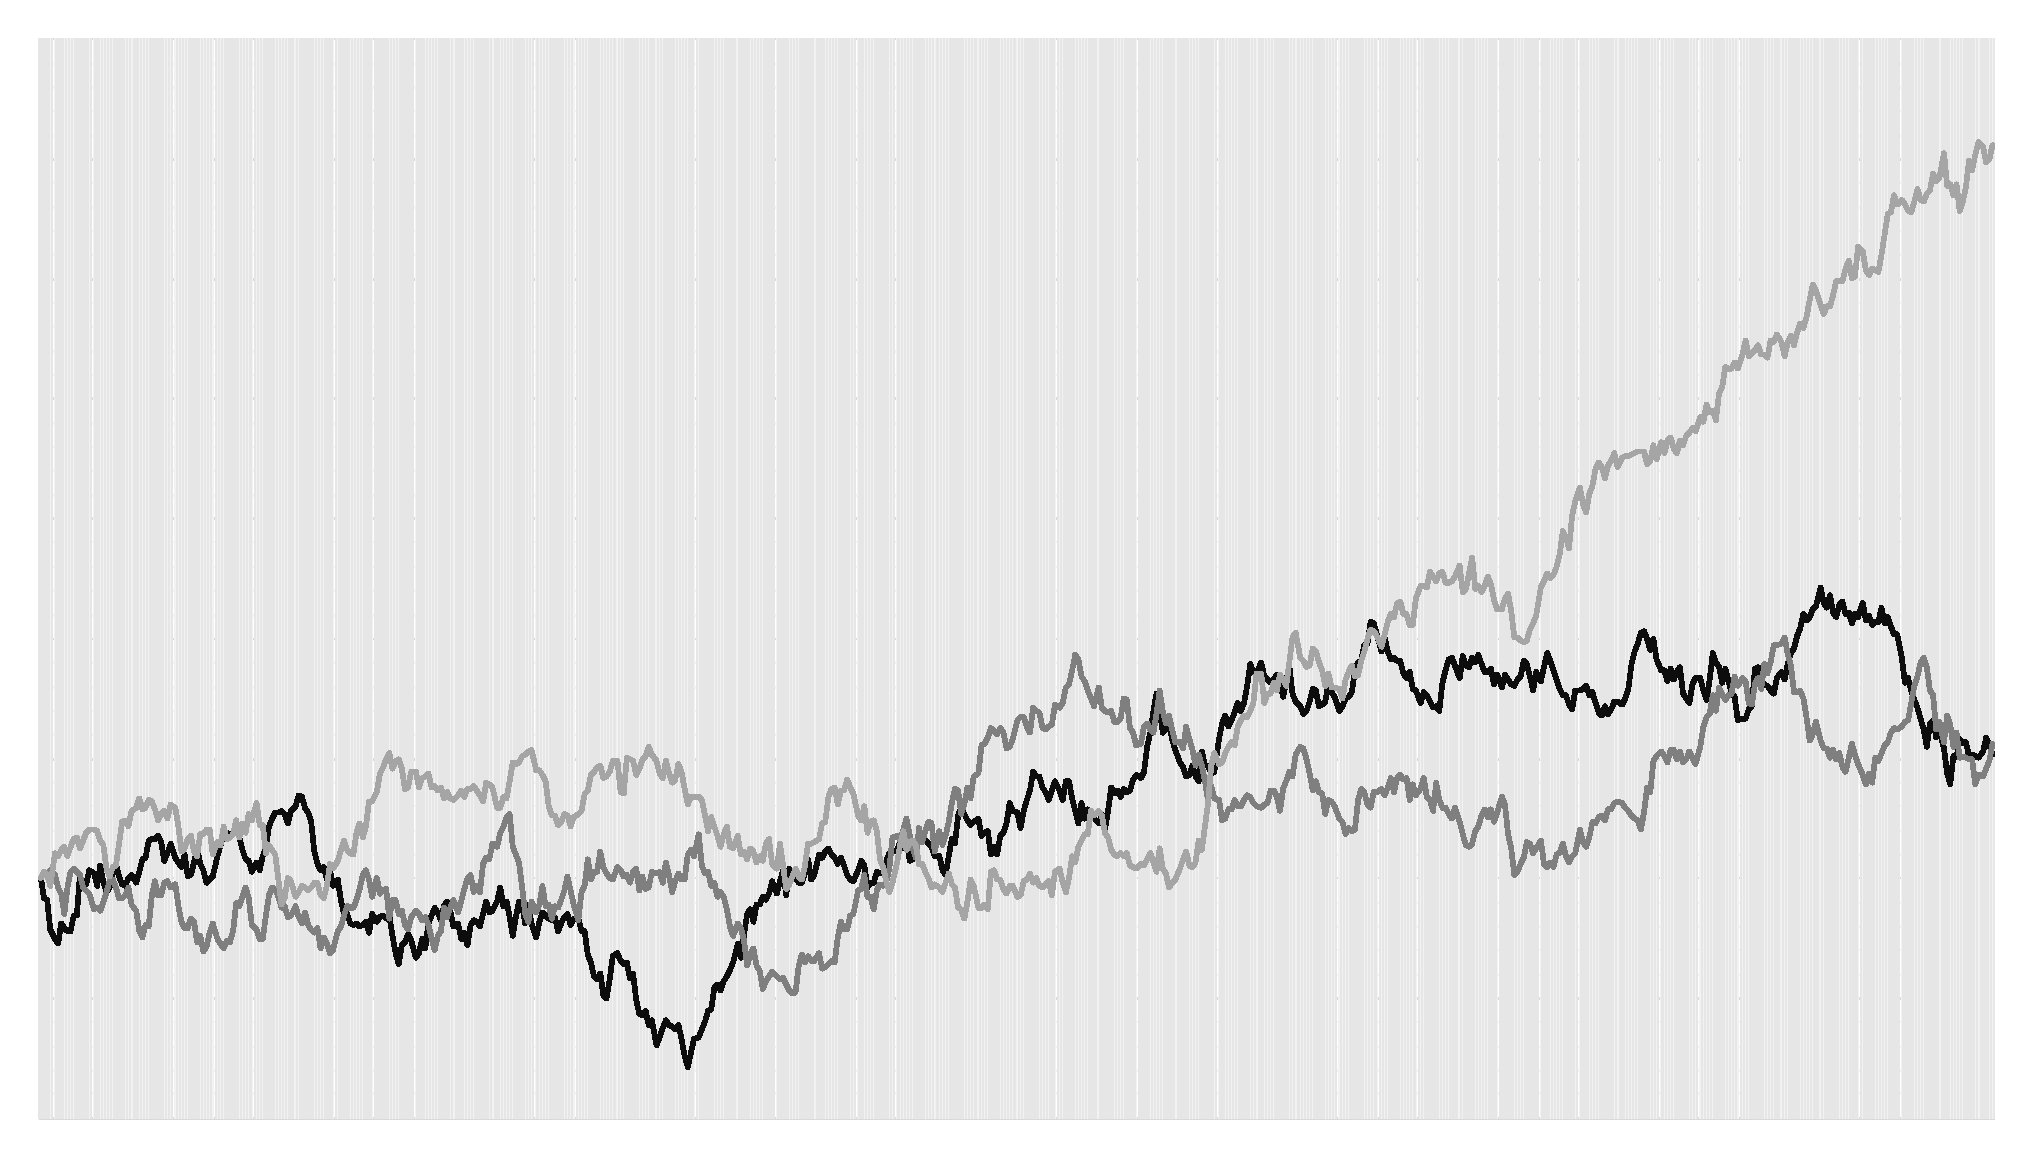
\includegraphics[width=0.75\textwidth]{bm.eps}
\end{flushright}
\end{figure}
\clearpage	% 进入内页
\begin{center}
	\Large{\sffamily\bfseries\thmheiti 编译日期: \today} \\ \vspace{1em}
	
\end{center}
\vfill

\begin{flushright} \small
	苏绚 \\
	素以为绚兮\\
	知其白守其黑为天下式\\
	%个人主页: \href{******}{******}
\end{flushright}
\vspace{1.5em}

%\cleardoublepage
\end{titlepage}
